 
\chapter{Experiments and Evaluation}
\label{ch:experiments}

\section{Experimental Setup}
\subsection{Architectural Setup}



\begin{figure}[h]
	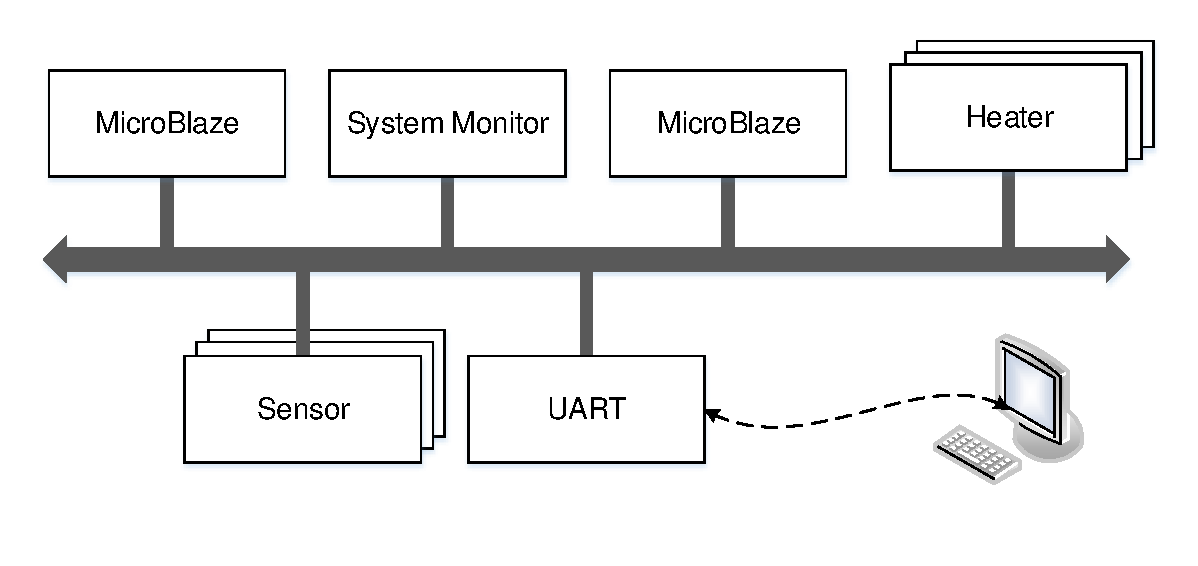
\includegraphics[width=\textwidth]{__pics/exsetup.pdf}
	\caption{ Architecture of the experimental setup }
	\label{pic:archsetup}	
\end{figure}

\subsection{System Setup}

LUTFF instead of LUT Osc --> why?

\begin{figure}[h]
	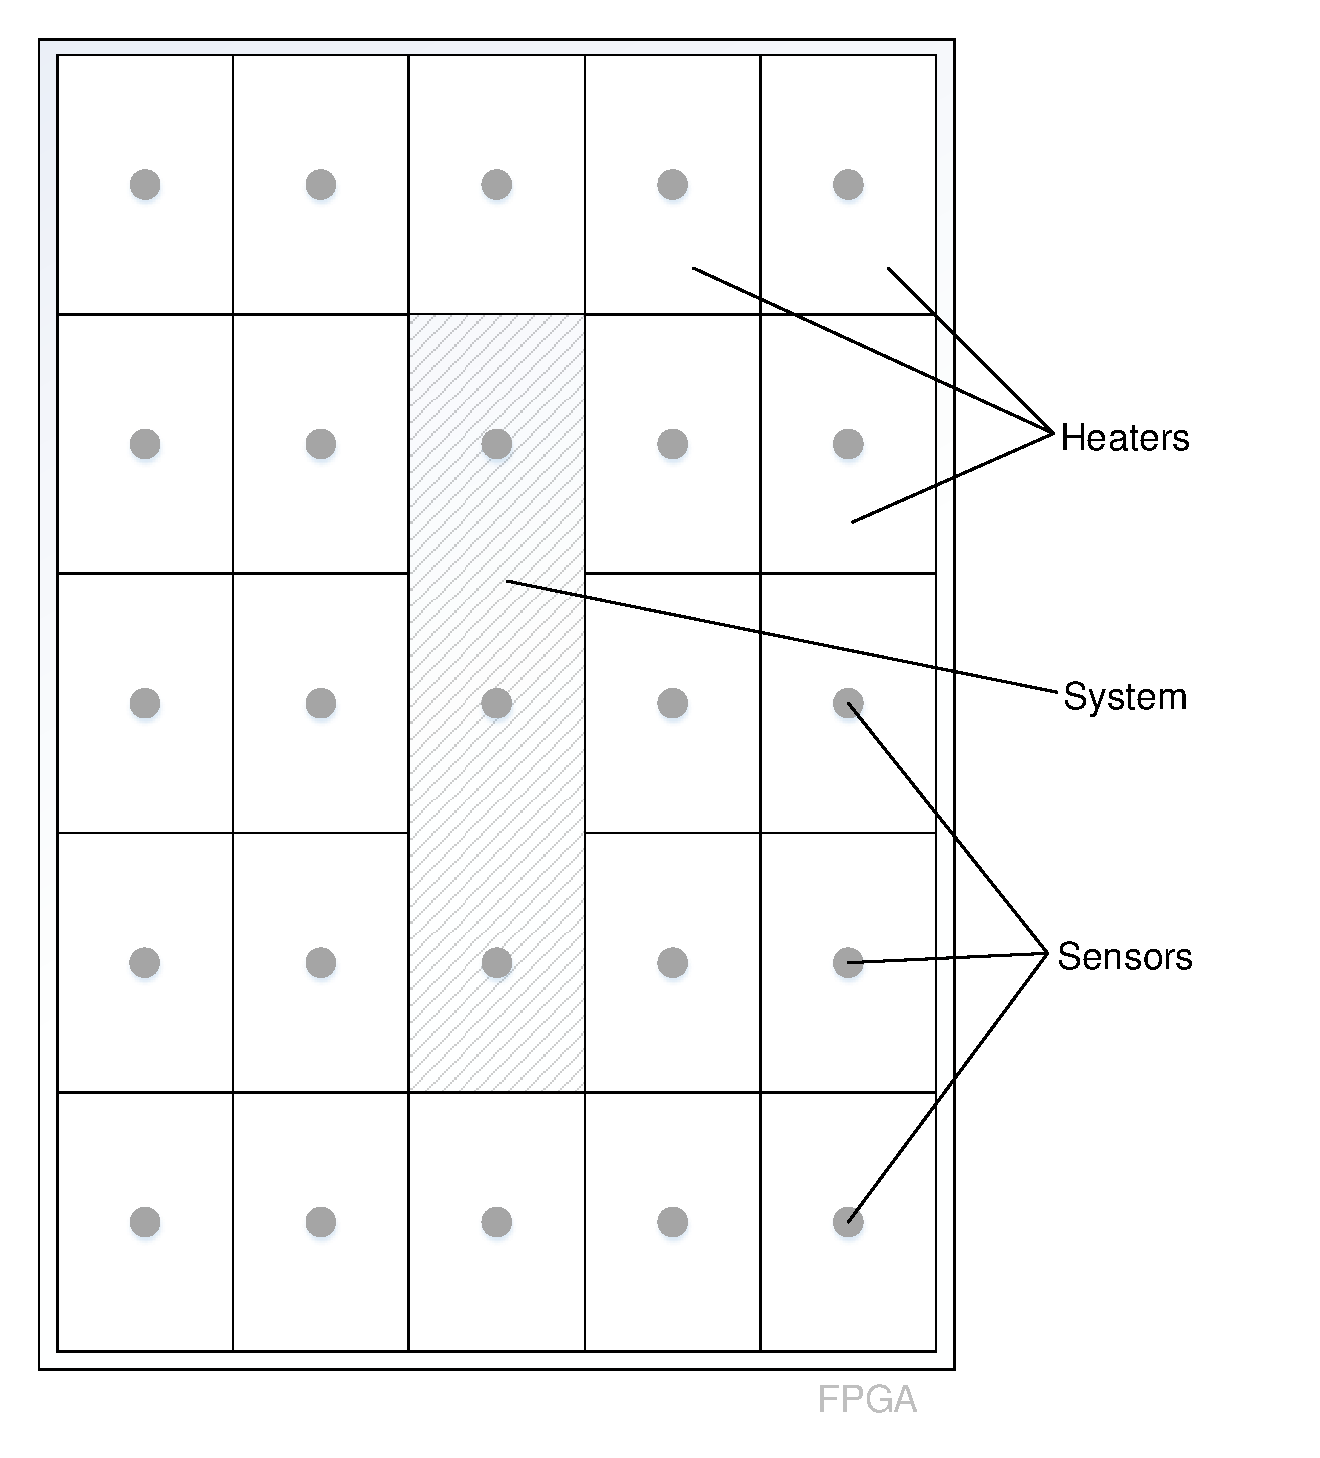
\includegraphics[width=\textwidth]{__pics/syssetup.pdf}
	\caption{ \ac{FPGA} experimental Setup}
	\label{pic:syssetup}	
\end{figure}

\begin{center}
	\begin{table}
		
		\begin{center}
			\begin{tabular}{|p{3.00cm}|p{6.48cm}|}
				
				\hline  \textbf{Time [min]} & \textbf{Heat Pattern}\\ 
				\hline \hline 0 -- 10 & All heaters activated\\ 
				\hline  10 -- 15 & Five upper heaters activated\\ 
				\hline  15 -- 20 & Five lower heaters activated\\ 
				\hline  20 -- 25 & Five leftmost heaters activated\\ 
				\hline  25 -- 30 & Five rightmost heaters activated\\ 
				\hline  30 -- 40 & Cool-down. No heaters activated\\ 
				\hline
			\end{tabular} 
			\caption{The different experiment's heat patterns}
			 \label{tab:heat_pattern}
		\end{center}
	\end{table}
	
\end{center}

\section{RC-Network}
\subsection{Model Definition}
\subsection{Model Training}
\subsection{Results for several Learning Algorithms}
\begin{itemize}
\item{Discussion of Convergence}
\item{Discussion of Accuracy}
\item{Discussion of On-Line Suitability}
\item{Discussion of Embedded Implementation}
\end{itemize}

\subsection{Model Behaviour}

\subsubsection{Behaviour at leveled final Temperature}
\subsubsection{Behaviour over Time}